\chapter{Integration of backward Monte Carlo software into
ICEDUST}
\label{app:bmc_integration}

% \begin{itemize}
%     \item External packages: PUMAS, GOUPIL, GOUPIL components. Cite~\cite{NIESS2022108438}.
%     \item Internal package: SimBackwardMC
% \end{itemize}


\section{Original implementation}
The backward Monte Carlo simulation software was originally written and applied
to the COMET Phase\nobreakdash-I experiment by Valentin Niess, author
of~\cite{Niess_Barnoud_Carloganu_Menedeu_2018,NIESS2022108438}.
Figure~\ref{fig:pumas_integration_strategy} shows the layout of the original set
of software layers used to run backward MC simulations in the Phase\nobreakdash-I world. 

At the core of the backward Monte Carlo simulation is the backward transport
engine, PUMAS~\cite{NIESS2022108438}. PUMAS is responsible for the propagation
of particles through matter and the computation of MC weights based on the path
taken and the interactions undergone, as discussed in
Section~\ref{sec:bmc_method}. Because it is designed exclusively for this
purpose, PUMAS does not provide utilities for navigating through complex
geometries or sampling the flux from pre-computed tables. Another package,
GOUPIL, takes on this role as an interface to PUMAS, and allows the user to
specify a geometry, a source flux, as well as the local topography and
geomagnetic field around the experiment's location. An additional interface
between GOUPIL and {\sc Geant4}, \texttt{goupil-geant4}, was developed to allow
the user to control backward MC runs with the {\sc Geant4} macro user interface
and to load and navigate the geometry from a GDML file. The final layer,
\texttt{resample-simg4}, provides a command-line interface and enables events
generated by \texttt{SimG4} to be read as input for the backward MC simulation
to estimate their flux.


\begin{figure}
    \centering
    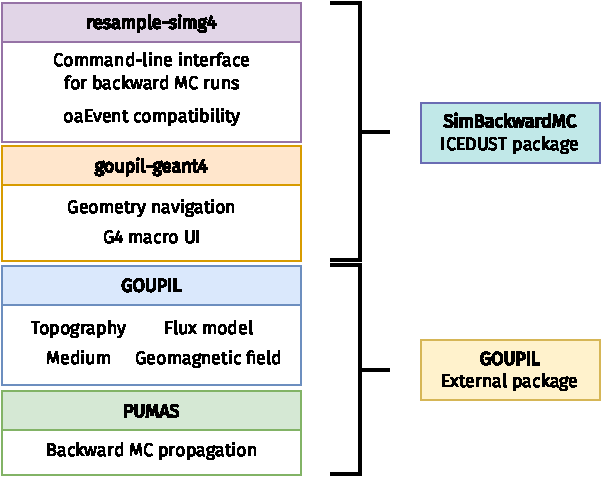
\includegraphics[width=0.6\textwidth]{appendixA/integration_strategy.drawio.pdf}
    \caption{ Software packages that compose the original backward MC simulation
        stack for the Phase\nobreakdash-I study, and organisation of their integrated
        ICEDUST counterparts.}
    \label{fig:pumas_integration_strategy}
\end{figure}

\section{Integration}

Figure~\ref{fig:pumas_integration_strategy} also shows how the original software
was arranged to become part of the ICEDUST framework. Since the PUMAS and GOUPIL
packages are unlikely to undergo quick iterative changes over time, they are integrated
into an external package. The functionalities of the upper two layers of the
stack are combined into a new ICEDUST package called \texttt{SimBackwardMC}.

The way in which the layers are organised is not the only difference between the
original and current software. Three major changes were implemented during the
integration in order to bring the original software closer to the ICEDUST
workflow.

\begin{itemize}
    \item {\bfseries Geometry format:} originally read from GDML files, the
    geometry is now created from the same classes and macro files that define
    the simulation world in forward MC runs by the \texttt{SimG4} package. This
    additionally ensures that the geometry used in forward and backward MC
    simulations is identical.
    \item {\bfseries Entry point:} the main \texttt{resample-simg4} entry point
    was previously a Lua script executed via LuaJIT which defined the
    command-line interface, configured the backward simulation run, and
    processed the output. \texttt{SimBackwardMC} uses a standard ICEDUST event
    loop executable as its entry point to handle command-line arguments, read
    events from input \texttt{oaEvent} files and output the results of the
    backward simulation.
    \item {\bfseries Output format:} \texttt{resample-simg4} wrote the results
    of backward sampling to a text file in a format similar to CSV.
    \texttt{SimBackwardMC} writes to a \texttt{RooTracker} file instead, since
    that is a standard ICEDUST format and a good fit to store the kinematics of
    processed events along with their estimated flux.
\end{itemize}

The integrated backward MC software presented here was used to obtain the
results of Chapters~\ref{ch:cosmics} and~\ref{ch:phase-I_study}. It is also
currently being used in the work of others, for instance to estimate the
atmospheric muon flux at various locations around the Phase\nobreakdash-I detector system
and validate the results with real measurements. Through our standardisation of
some parts of the original software and the addition of specific documentation,
we hope that the \texttt{SimBackwardMC} package will remain a readily accessible
tool for future cosmic ray studies in COMET.
